%%%%%%%%%%%%%%%%%%%%%%%%%%%%%%%%%%%%%%%%%%%%%%%%%%%%%%%%%%%%%%%%%%%%%%%%%%%%%%%%%%
%%      Template using LaTeX  Tutorial tex files								%%
%%      																		%%
%%      Copyright Rho Vector Latex Tutorial 2021								%%
%%		rhovector <rhovector@gmail.com>			 								%%
%%		vivekadi <vivek.adishesha@gmail.com>,									%%
%%		chiranjitpatel <chiranjitpatel08@gmail.com>								%%
%%																				%%
%%																				%%	
%%      This program is FREE SOFTWARE; you can redistribute it and/or modify	%%
%%      it under the terms of the GNU General Public License as published by	%%
%%      the Free Software Foundation; either version 2 of the License, or		%%
%%      (at your option) any later version.										%%
%%      																		%%
%%      This program is distributed in the hope that it will be useful,			%%
%%      but WITHOUT ANY WARRANTY; without even the implied warranty of			%%
%%      MERCHANTABILITY or FITNESS FOR A PARTICULAR PURPOSE.					%%
%%      See GNU General Public License for more details.						%%
%%      																		%%
%%      You should have received a copy of the GNU General Public License		%%
%%      along with this program; if not, write to the Free Software				%%
%%      Foundation, Inc., 51 Franklin Street, Fifth Floor, Boston,				%%
%%      MA 02110-1301, USA.														%%
%%%%%%%%%%%%%%%%%%%%%%%%%%%%%%%%%%%%%%%%%%%%%%%%%%%%%%%%%%%%%%%%%%%%%%%%%%%%%%%%%%


\documentclass{article}

%% Package "graphicx" is useed to place and manipulate images in the document %%
\usepackage{graphicx}

%% Package "rotating" for image rotation %%
\usepackage{rotating}

%% Package "float" for parameters to locate the images %%
\usepackage{float}

\begin{document}
	
	%% Image can also be added by copying the image from any folder and paststing it here (CTRL + V)  %%
	
	%% Adding Figure, captions and label with "figure" block %%
	\begin{figure}[h!]											%% Float parameter for image position on page %%
		\centering												%% Center justification of image %%
		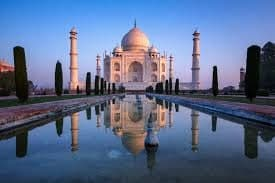
\includegraphics[width=0.8\textwidth]{images/taj.jpg}   %% width = This is the width of figure box %%
		\caption{Taj Mahal}										%% name of the figure %%
		\label{taj}												%% figure reference label %%
	\end{figure}

	%% In line inclusion of figure %%
	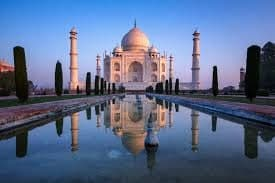
\includegraphics[width=0.4\textwidth]{images/taj.jpg}\\  

	%% \label{fig:mesh1} 
	%% This will set a label for this figure. Since labels can be used in several types of elements within the 		%% document, it's a good practice to use a prefix, such as fig: in the example.
	%% \ref{fig:mesh1}

	%% Rotating Image Method-1 %%
	%% In this method the image is rotated, but the caption is retained in the same text direction %%
	\begin{figure}[h!]
		\centering
		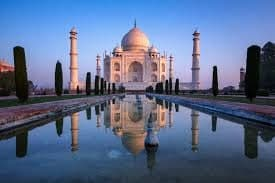
\includegraphics[width=1\textwidth, angle=90]{images/taj.jpg}    %% rotation of image by 90 degrees %%
		\caption{Taj Mahal rotated 90 deg}
		\label{tajrot90}
	\end{figure}

	%% Rotating Image Method-2 %%
	%% Using sidewaysfigure, this rotates the caption also along with the image %%
	\begin{sidewaysfigure}[h]
		\centering
		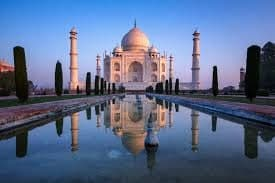
\includegraphics[width=1\textwidth]{images/taj.jpg}    %% rotation of image by 90 degrees %%
		\caption{Taj Mahal rotated 90 deg with text}
		\label{tajrot90_side}
	\end{sidewaysfigure}


	%% Define the width and the height of the picture. You can use different units for these parameters. %%
	%% If only the width parameter is passed, the height will be scaled to keep the aspect ratio. %%
	%% Height parameter %%	
	\begin{figure}[h!]
		\centering
		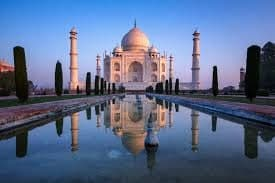
\includegraphics[height=0.8\textwidth]{images/taj.jpg}
		\caption{Using the height parameter}
	\end{figure}

	%% Float Parameters %%
	Float Parameters for Image locations (Use Float Package in package call section)
	\paragraph
	h - Place the float here.\\
	t - Position at the top of the page.\\
	b - Position at the bottom of the page.\\
	p - Put on a special page for floats only.\\
	! - Override internal parameters LaTeX uses for determining "good" float positions.\\
	H - Places the float at precisely the location in the LATEX code. Requires the float package
	
	
	%% Image reference "\ref{fig:image_name}" %% 
	Construction of the mausoleum was essentially completed in 1643, but work continued on other phases of the project for another 10 years. Depicted in the \textit{Figure} \ref{tajrot90}.
	
	

\end{document}